\documentclass{uark}

%recommended packages
\usepackage{amsmath} %better math handling
\usepackage{mathcomp} %don't remember why I include this
\usepackage{graphicx} %used for figures
\usepackage[version=3]{mhchem} %used for chemical formulas, in text and in eq.
\usepackage{siunitx} %used to easily format numbers with units, including greek

\usepackage{subfig}
\usepackage{csquotes}
\usepackage{float}

\begin{document}
\bibliographystyle{IEEEtran}

%FRONT MATTER
\title{Smart-Insect Monitoring System Integration and Interaction via \\
AI Cloud Deployment and GPT}

\author{Ahmed Moustafa}
\degreeyear{2023}

\degreetitle{Bachelor of Science} 

\field{Computer Science}
\chair{Dr. Khoa Luu}
\othermembers{
Dr. John Gauch, CSCE\\
Dr. Alexander Nelson, CSCE\\ 
}
\numberofmembers{3} 

\abstract{ 
The Insect Detection Server was developed to explore the deployment and integration of an Artificial Intelligence model for Computer Vision in the context of insect detection. The model was developed to accurately identify insects from images taken by camera systems installed on farms. The goal is to integrate the model into an easily accessible, cloud-based application that allows farmers to analyze automatically uploaded images containing groups of insects found on their farms. The application returns the bounding boxes and the detected classes of insects whenever an image is captured on-site, enabling farmers to take appropriate actions to address the issue of the insects' presence.
To extend the capabilities of the application, the server is linked to a GPT-3.5 API. This will allow users to ask questions about the bugs detected on their farms, creating an ``online expert"-like feature. Python, C++, and Computer Vision libraries were used for the detection model, while the OpenAI API was used for GPT-3.5's integration. By combining these technologies, farmers can more effectively and efficiently manage pests on their farms than current alternatives. This Generative Pre-trained Transformer (GPT) aspect of the project can be leveraged to enable the emulation of agricultural experts for users/farmers. The large language model (LLM) neural network can be fine-tuned using prompt engineering to generate natural language responses to user queries. This will enable farmers to get expert advice and guidance on pest management without having to consult with a human expert. The integration of GPT-3.5 API will also allow the application to provide personalized recommendations based on each farm's specific needs and circumstances. This added feature will give the farmers a more comprehensive and tailored approach to pest management, further increasing the efficiency and effectiveness of their pest control strategies.
The significance of this research lies in the development of a practical and accessible tool for farmers to manage pests on their farms. Using Computer Vision and Artificial Intelligence, farmers can quickly and accurately identify insects, leading to more efficient and effective pest management. This could help farmers reduce the use of pesticides and other forms of pest management, leading to improved crop yields and reduced environmental impacts. The potential benefits of this technology extend beyond the agricultural industry, as the techniques used in this research can be applied to a wide range of computer vision and user-facing data analytic applications. For example, the developed techniques could be applied to other fields, such as surveillance, security, and medical imaging.
}

\begin{frontmatter}
\makefrontmatter 

\begin{acknowledgements} 
I want to express my sincere gratitude to several individuals and institutions who have played a crucial role in the completion of this thesis. First and foremost, I would like to thank Dr. Khoa Luu, my honors research mentor, for his invaluable guidance, support, and mentorship throughout the entire research process. Dr. Luu's expertise, insights, and constructive feedback have been instrumental in shaping this work and in helping me develop as a researcher. I would also like to extend my thanks to Thanh-Dat Truong, the graduate student and fellow researcher in the Computer Vision and Image Understanding (CVIU) lab who generously shared his time and expertise to help with the model and project as a whole. Dat's contributions were essential to the success of this research, and I am very grateful for his support. I am also indebted to the University of Arkansas for providing the resources and opportunities necessary to facilitate this Undergraduate Honors Research. The university's commitment to fostering undergraduate research has been instrumental in my academic and professional development, and I am honored to have been a part of this program. Finally, I would like to thank my thesis defense committee members, Dr. Khoa Luu, Dr. John Gauch, and Dr. Alexander Nelson, for their time and expertise.
\end{acknowledgements}

\tableofcontents
\listoffigures
% \listoftables   % Uncomment if you have any tables TABLES 

\newpage


\end{frontmatter}

%BODY
%The point of including each chapter is because once the chapters get filled up it takes a while to execute the whole file. This way, you can comment out each file except the one you are working on to save compile time when checking.
\chapter{Introduction}

The U.S. agricultural industry has long been a cornerstone of the country's economy, contributing over a trillion dollars in value-added to the GDP annually. Specifically, farms generate approximately \$164.7 billion annually, as illustrated in Fig \ref{fig:1.1} \cite{zahniser_kassel_2023, depietro_2022}. One of the significant challenges farmers face is managing pests and crops, with the average cost being approximately ``34\% of a farmer's variable crop production costs" \cite{lrichmond_2007}. While pests can cause economic loss and harm to farmland, there are also beneficial insect species that save growers millions of dollars annually \cite{state_2010}.

\begin{figure}[H]
\begin{center}
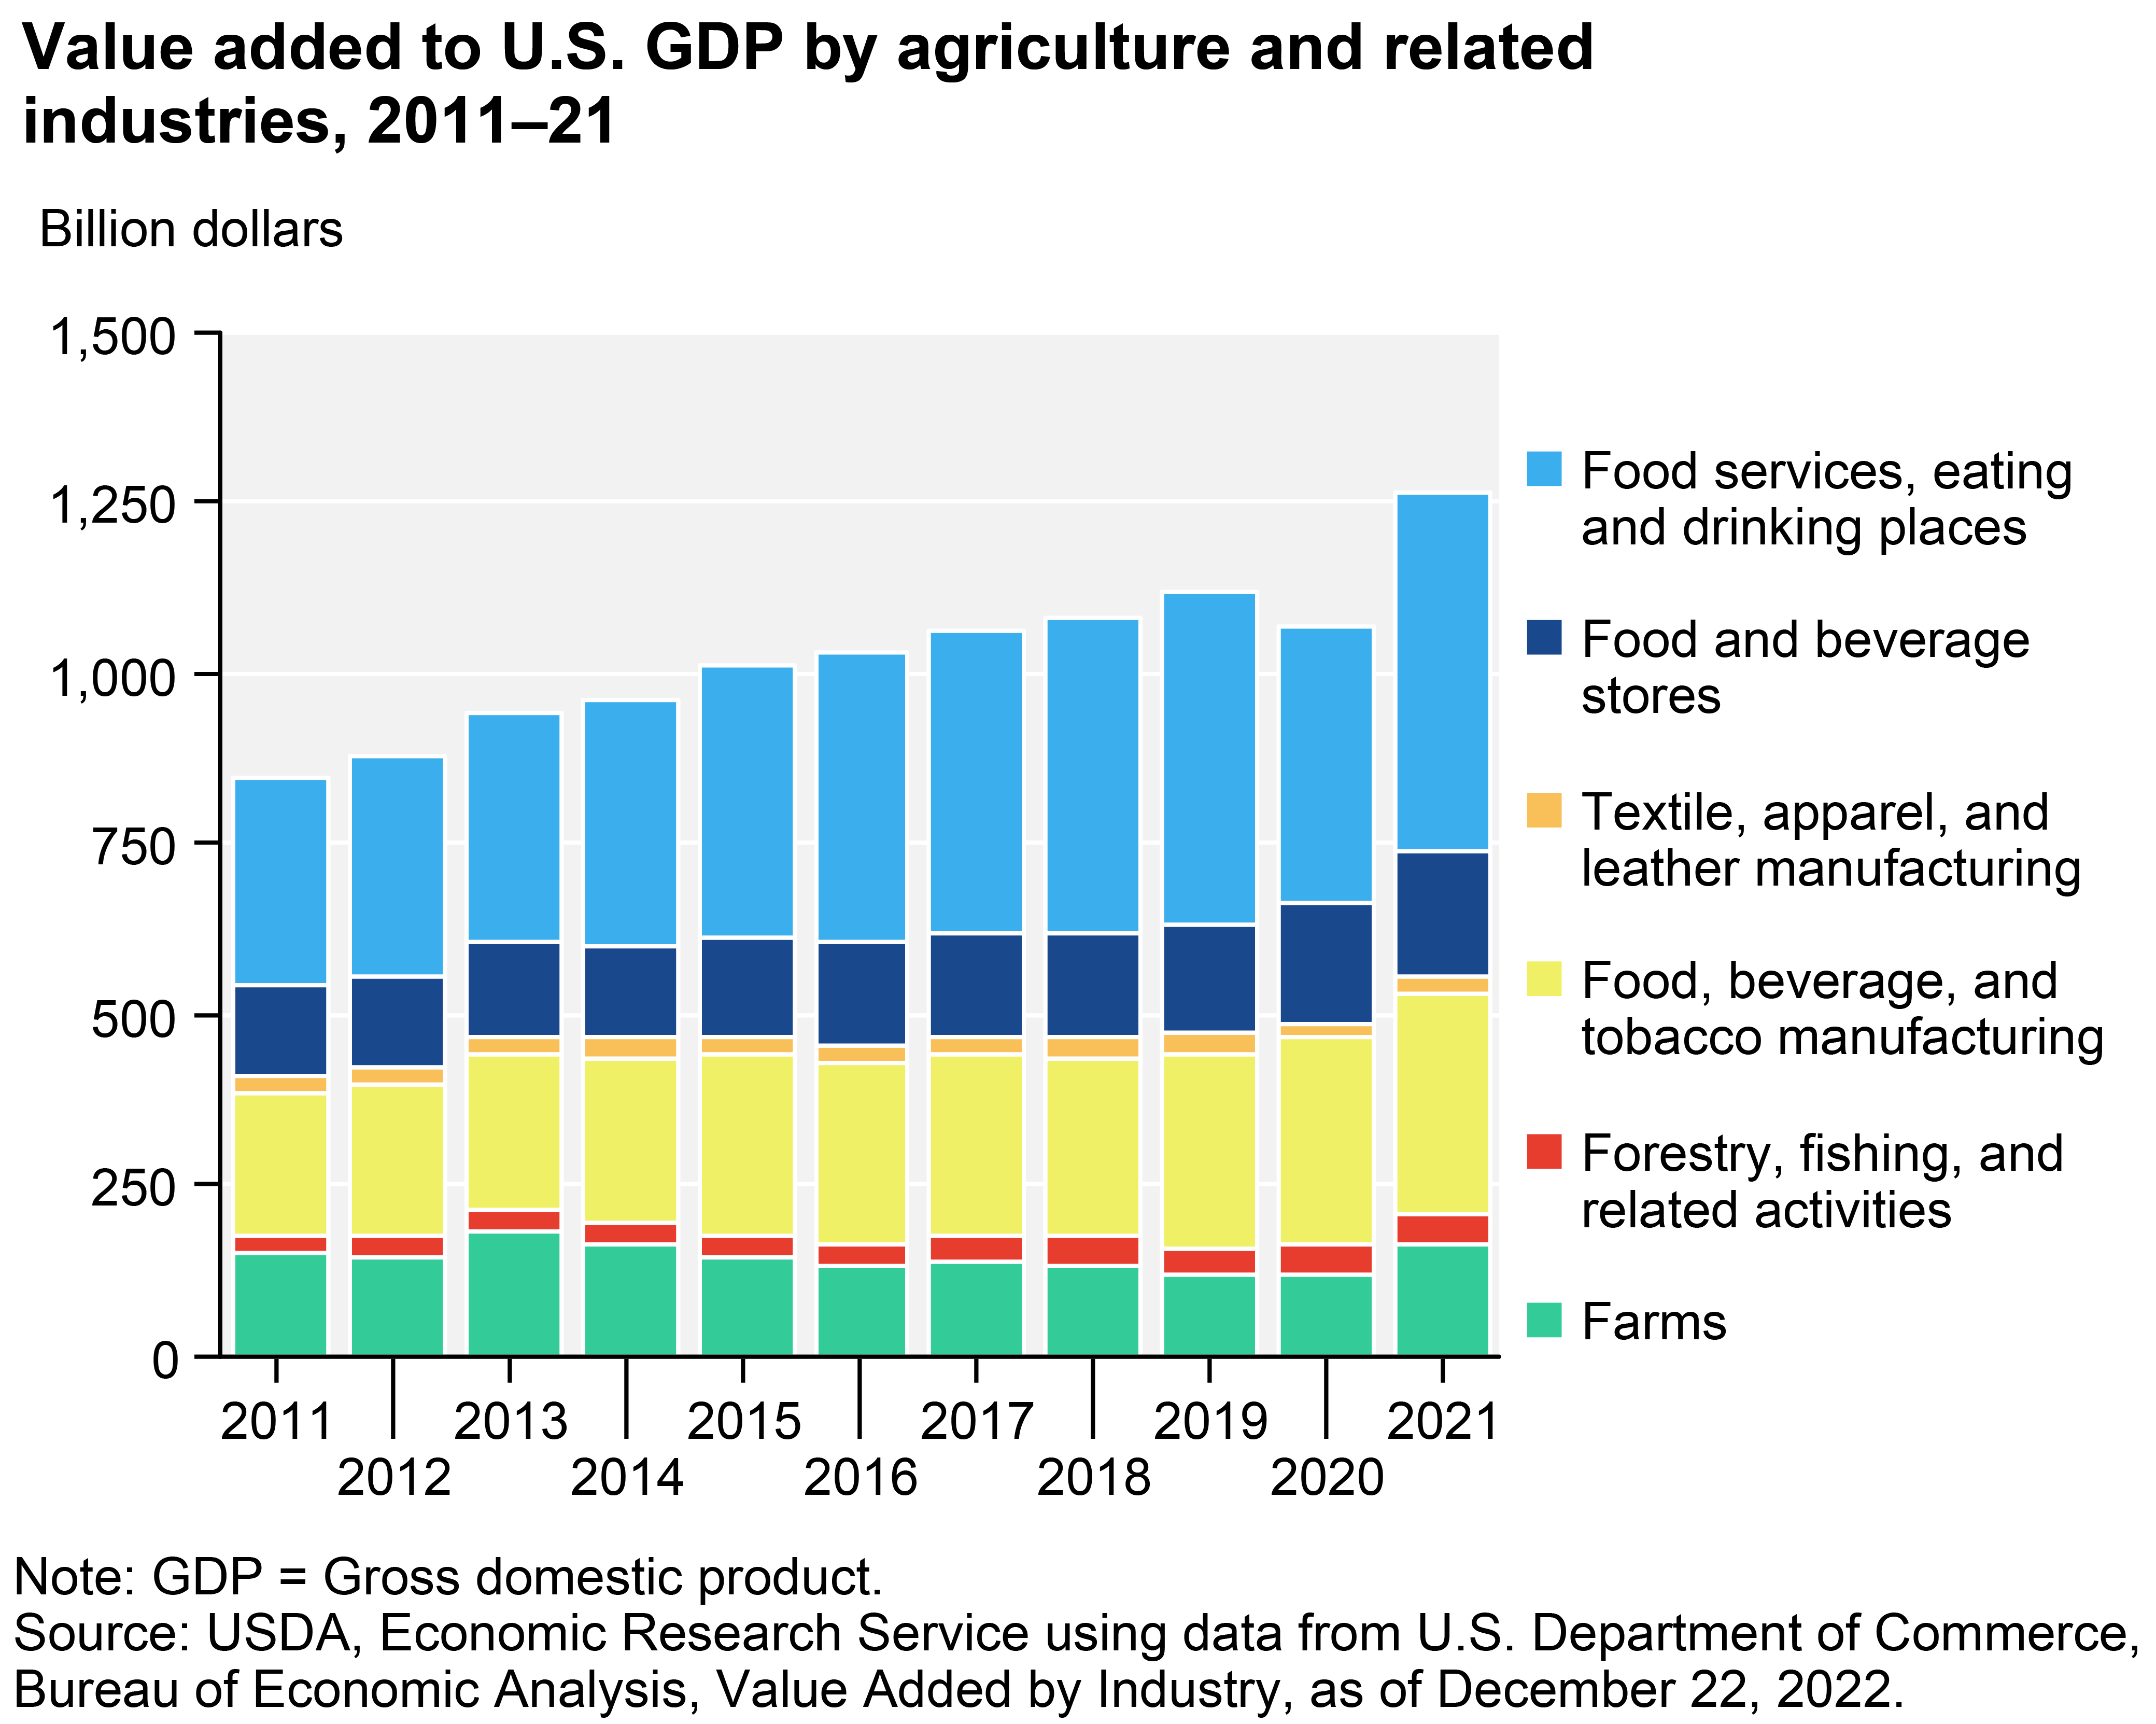
\includegraphics[width=0.85\linewidth]{Honors_Thesis/Figures/1.1.png}
\end{center}
\caption{Chart displaying the value added to U.S. GDP by Agriculture and related industries, 2011-21. Farms alone exceed \$150 billion annually.}
\label{fig:1.1}
\end{figure}

To account for rising number of pests and invasive species over the past century, farmers have increased their pesticide use to match, as seen in Fig \ref{fig:1.2} \cite{nehring_fernandez-cornejo_vialou_martin_wechsler_osteen}. Besides increased costs, the consequences of this rise in pesticide usage include unintentional environmental and human harm due to runoff and unintended targets \cite{aktar_sengupta_chowdhury_2009}. Another risk related to classic pesticide usage is the development of insecticide resistance through surviving insect populations and mutations \cite{gut_mcmanus_isaacs_schilder}. With this many risks associated with traditional pesticide use, adding more quantity can lead to diminishing returns on pesticide efficacy and even negative returns in extreme cases.

\begin{figure}[H]
\begin{center}
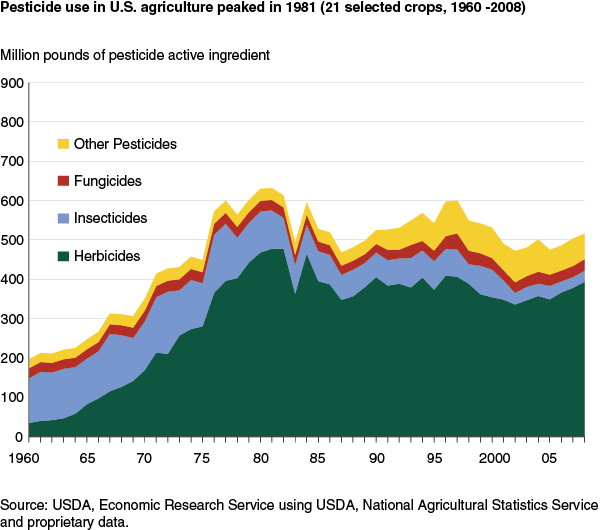
\includegraphics[width=0.9\linewidth]{Honors_Thesis/Figures/1.2.png}
\end{center}
\caption{Chart displaying the rise and fall of pesticide usage in the U.S. with a peak in 1981, 1960-2008.}
\label{fig:1.2}
\end{figure}

To combat the rise in pesticides we see in Fig \ref{fig:1.2} due to classic pest control methodologies, farmers began planting new pest-resistant strains of crops and implemented Integrated Pest Management (IPM). IPM is a pest control strategy that prioritizes long-term prevention through environmentally considerate methods. These methods include manipulating the pests' habitat, replacing possibly outdated practices by the farmer, planting resistant crop varieties, etc. Though there are many different IPM practices, all IPM programs contain the same six general components \cite{ipm}:

\begin{displayquote}
\begin{enumerate}
   \item Pest identification
   \item Monitoring and assessing pest numbers and damage
   \item Guidelines for when management action is needed
   \item Preventing pest problems
   \item Using a combination of biological, cultural, physical/mechanical and chemical management tools
   \item After action is taken, assessing the effect of pest management 
\end{enumerate}
\end{displayquote}

IPM is becoming increasingly adopted among farmers to reduce costs and yield losses. A concise version of an IPM is illustrated in Fig \ref{fig:1.3} \cite{hardy_lesher_olson_2021}. The limitation of many IPMs is their labor constraints, as the identification and monitoring of pests require consistent manual sampling, inspection, and expertise regarding insects \cite{zehnder_2009}. A novel system combining modern hardware and software has been developed to address these challenges to create a consistent and efficient pest identification and monitoring method.

\begin{figure}[H]
\begin{center}
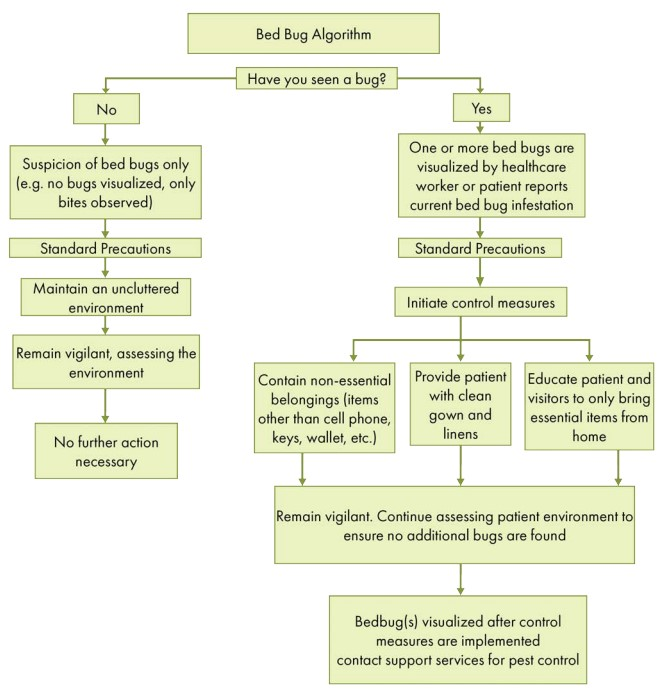
\includegraphics[width=0.95\linewidth]{Honors_Thesis/Figures/1.3.jpg}
\end{center}
\caption{Bed Bug Algorithm: small-scale Integrated Pest Management (IPM) plan.}
\label{fig:1.3}
\end{figure}

Integrating an on-site camera system running an insect detection and classification model with a user-facing application can revolutionize farmers' management of pests. By leveraging Artificial Intelligence, farmers can take informed action and track pest numbers in real-time, thereby improving the sustainability of IPM plans and increasing the efficiency of pest management. Furthermore, the system is complemented by the integration of an additional AI model that is used to emulate an agriculture expert: OpenAI's GPT-3.5. This feature provides farmers with personalized recommendations based on their unique farm conditions, allowing for faster and more effective pest control strategies. This innovative approach can potentially reduce the use of harmful pesticides and improve crop yields by a significant amount.



\chapter{Related Works}
Currently, a majority of farmers and insect researchers manually sample insects regularly. Since many insects and mites can be tiny, the samplers must carry tools like digital cameras and 10x magnifying glasses. This monitoring procedure will include traps, beating counts, fecal pellet collection, and more \cite{pinkston}. Though these procedures are successful, maintaining the sampling schedule is troublesome since the researcher/farmer must use different techniques and traps for various insects. For example, to detect and monitor populations of alfalfa weevils, armyworms, and leafhoppers, the recommended guidelines are to do a sweep-net sample twice a week or more \cite{long_goodell_2017}. Moreover, manual sampling can be prone to errors and biases, resulting in inaccurate insect population estimates. Researchers or farmers may miss small insects or misidentify them, leading to incorrect population counts. Additionally, the accuracy of the estimates can be affected by the sampling frequency, location, and timing, as well as the experience of the sampler. These manual sampling limitations can result in delays and errors in the Integrated Pest Management plan.

The Agricultural industry is known for its innovation as farming has improved throughout history for the sake of efficiency. Original manual labor was replaced with machines that increased harvest yields and decreased time spent on many farming processes, including planting, maintenance, and harvesting. Recent advancements in robotic agricultural technology have resulted in the creation of automated harvesting systems that use Deep Learning, sensor-map fields, etc., to replace some of the many manual aspects of agriculture \cite{magee_2020}. Although this principle of automation and technological advancement is exceptionally efficient, it often needs to account for issues like pest control which may be external to the base processes like seeding, growing, and harvesting of arable land.

\section{Automated Farm Management}
Automated farm management systems have expanded their scope to encompass pest monitoring and control, increasing efficiency and accuracy. For instance, Zhang et al. \cite{zhang_bu_wang_2022} developed a system that uses deep learning to identify and count insects on crops within a greenhouse. The system utilizes cameras to capture images and processes them with a convolutional neural network, providing real-time pest data to farmers. This method has the advantage of offering continuous monitoring but may be limited by factors such as camera resolution and lighting conditions. Similarly, an automated pest detection system for crops using unmanned aerial vehicles (UAVs) equipped with cameras and a machine learning-based classification algorithm was proposed, as shown in Fig \ref{fig:2.1} \cite{10.3389/fagro.2021.640885, app13031851}. This approach enables large-scale monitoring and rapid response to pest infestations but may be affected by environmental factors such as wind and weather.

\begin{figure}[H]
\begin{center}
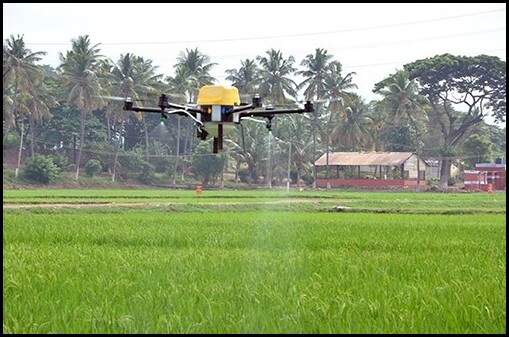
\includegraphics[width=0.85\linewidth]{Honors_Thesis/Figures/2.1.jpg}
\end{center}
\caption{Hexacopter spraying pesticides in Tamil Nadu Agricultural University Farm rice fields in Tamil Nadu, India, during October 2019.}
\label{fig:2.1}
\end{figure}

Additionally, ``Internet of Things" (IoT) based systems have been employed to improve pest management. Qazi et al. \cite{9716089} mention examples of IoT-based smart agriculture systems that integrate pest monitoring with other farm management tasks, such as soil and climate monitoring. By consolidating multiple aspects of farm management, these systems enable an increase in informed decision-making and rapid interventions. However, implementing IoT systems may require significant upfront investment and technical expertise, which may be a barrier for small-scale farmers.

Recent advancements in remote sensing technology have also been employed in pest detection and monitoring. There is an example where remote sensing was used to detect insects in agriculture, focusing on the spectral characteristics of insect sounds \cite{mankin_mccoy_flanders_brandhorst_crocker_shapiro}. This approach can help identify and localize insects in the field but might be limited by the complexity of the acoustic environment and the need for extensive insect sound libraries.

\section{Detection and Classification}
Recent advances in AI and computer vision have facilitated the development of more sophisticated detection and classification methods for insect monitoring. There are examples of efficient deep learning-based approaches being used for detecting and classifying insects through convolutional neural networks (CNNs) \cite{insects14020148}. This method accurately recognizes various insect species, including pests and beneficial insects. However, the performance of such models may be limited by the quality and diversity of the training data, which could lead to misclassifications.

Thenmozhi et al. \cite{THENMOZHI2019104906} developed an automatic recognition system for insect pests using image processing techniques and machine learning classifiers. This approach achieved high recognition rates but required manual preprocessing of images for feature extraction, which could be time-consuming and labor-intensive.

\section{Support Tools}
The emergence of AI-driven support tools has provided farmers and researchers with valuable resources for making educated choices in pest control. Navarro-Hellin et al. \cite{NAVARROHELLIN2016121} created a decision support system that integrates pest monitoring information, meteorological data, and crop growth simulations to deliver customized pesticide application guidance. This system encourages eco-friendly pest management by reducing pesticide use and optimizing crop production.

A pest risk prediction system based on deep learning and remote sensing data was proposed by Chen et al. \cite{CHEN2022107302}. The system predicts the likelihood and severity of pest outbreaks, allowing farmers to implement preventative actions and reduce the consequences of pest infestations. Nevertheless, the precision of these models may be affected by the quality and promptness of input data and the intricacy of the factors that contribute to pest behavior.

Mimicking expert knowledge and decision-making has been an area of interest in research and development across various sectors. Expert systems have been created to help users with tasks that would usually necessitate the skills of a professional, such as medical diagnoses, financial planning, and legal counsel. These systems often employ AI, machine learning, and natural language processing to enable expert-like decision-making and deliver tailored recommendations \cite{durkin1994expert, charniak_mcdermott_1988}.

Expert emulation has been applied to various areas, including pest management in agricultural settings. Gonzalez-Andujar \cite{jose_article}, for example, designed an expert system to estimate the risk of insect pests in olive crops. This system uses specialized knowledge to offer personalized pest management advice based on user-provided information, like plant species and geographic location. Similarly, an expert system for assessing pest risk in organic agriculture was created that assists farmers in recognizing potential hazards and executing suitable pest management tactics \cite{MCKINION198531}.

In addition to conventional expert systems, chatbots have been utilized to replicate expert guidance and offer support in different industries. For instance, Agil-Ifdillah et al. \cite{reset.org_2022} created a chatbot to help farmers identify crop diseases and pests while providing expert suggestions on prevention and treatment methods. This approach enables farmers to access expert knowledge in a more accessible and user-friendly way, lowering the obstacles to adopting sophisticated pest management techniques.



\chapter{Background}
Artificial Intelligence has advanced at a remarkable rate recently, with Deep Learning models achieving state-of-the-art performance in various tasks. These models, which include Transformers, Convolutional Neural Networks (CNNs), and Generative Pretrained Transformers (GPTs), have been applied to a wide range of applications, including Natural Language Processing (NLP) and Computer Vision. This chapter provides an overview of the critical concepts and architectures underpinning these models and their applications in the on-site insect detection and classification system. The chapter also discusses prompt engineering, a technique used to optimize the performance of language models like GPT.

\section{Transformers}
Transformers are a type of Deep Learning Neural Network architecture \cite{transformers_1}. They have become the foundation for many state-of-the-art NLP and Computer Vision models. The primary value of the new transformer architecture is its ``self-attention mechanism," which enables selection across multiple inputs based on importance when processing each element. This mechanism enables transformers to effectively capture long-range dependencies and relationships in the input data.

Transformers have been widely used for machine translation, language modeling, and text classification. The Transformer architecture has an encoder and decoder component, each composed of multiple layers of self-attention and feedforward neural networks. The encoder takes in the input sequence for processing, and the decoder creates the output sequence. The generic model architecture of a Transformer developed by Google is shown in Fig \ref{fig:3.1}.

\begin{figure}[H]
\begin{center}
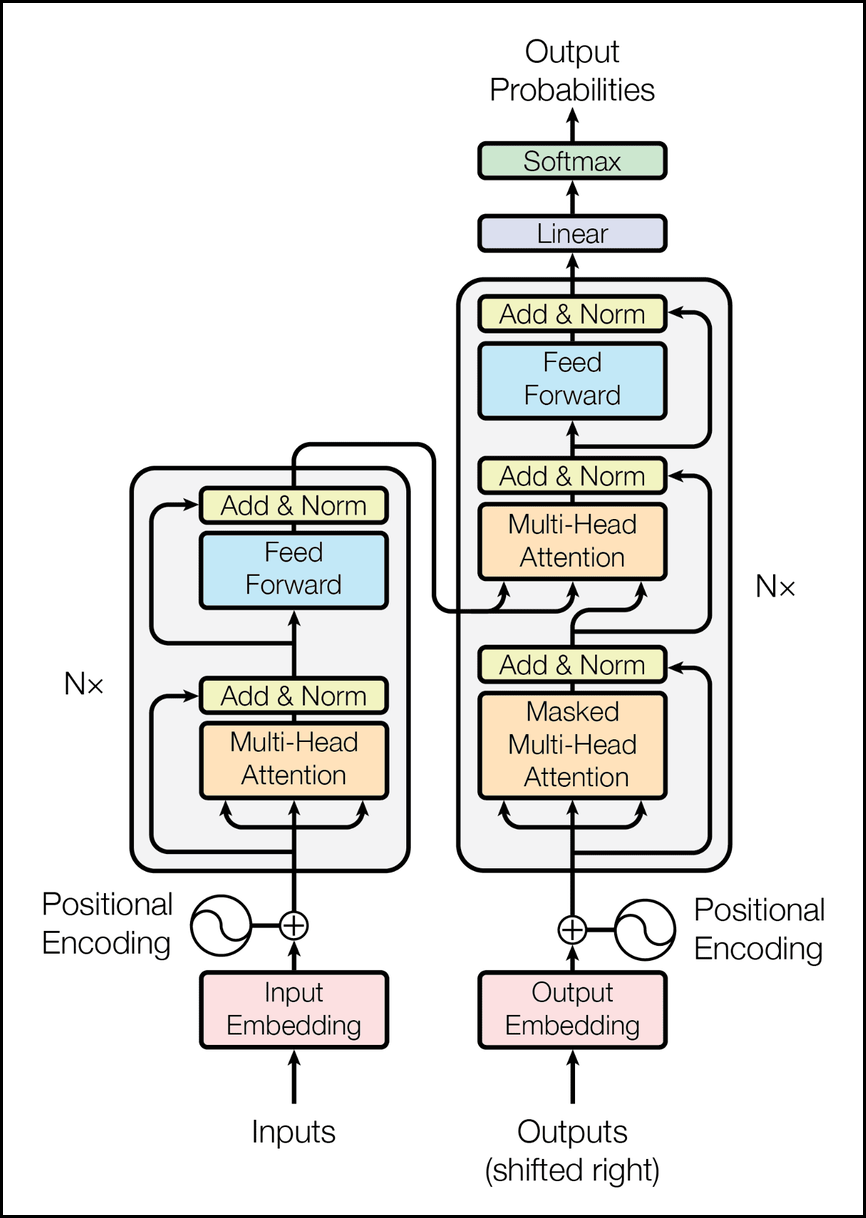
\includegraphics[width=0.85\linewidth]{Honors_Thesis/Figures/3.1.png}
\end{center}
\caption{The Transformer - model architecture \cite{transformers_1}.}
\label{fig:3.1}
\end{figure}

\section{Computer Vision Model}
The on-site insect detection and classification system leverages the power of deep learning models to achieve accurate and efficient results. By building upon previous research in the field of Computer Vision, the system employs a combination of detection and classification models to identify and categorize insects in images captured by the camera. The use of transformers in the computer vision domain allows the system to capture complex patterns and relationships in the image data, leading to high levels of accuracy and reliability. The following sections cover the details of the deep learning models and techniques used in the system.

\subsection{Deep Learning}
Within the field of Machine Learning exists its subset, Deep Learning, which involves the training of Neural Networks with many layers to perform tasks such as image and speech recognition \cite{lecun_bengio_hinton_2015}. A specific type of Deep Learning model used in Computer Vision is Convolutional Neural Networks (CNNs). CNNs consist of convolutional layers that automatically learn spatial rankings of features from the input data.

The ImageNet classification challenge has been a driving force behind developing Deep Learning models for Computer Vision. Notably, the AlexNet architecture \cite{NIPS2012_c399862d} achieved a breakthrough in the ImageNet challenge using deep CNNs. YOLO (You Only Look Once) is another popular deep learning model for real-time object detection and classification \cite{redmon2016}. What makes YOLO more efficient than traditional methods is its ability to process the entire inputted image in one go rather than multiple possessions. YOLO employs a single CNN that divides the input image into a grid and predicts each grid cell's bounding boxes and class probabilities. The model then thresholds these predictions to produce the final object detections.

Vision transformers \cite{DBLP:journals/corr/abs-2010-11929} are a recent development that applies transformer architecture to computer vision tasks. They divide an image into fixed-size patches and process them as a sequence using self-attention mechanisms. The model architecture of a Vision Transformer developed by Google is shown in Fig \ref{fig:3.2}.

\begin{figure}[H]
\begin{center}
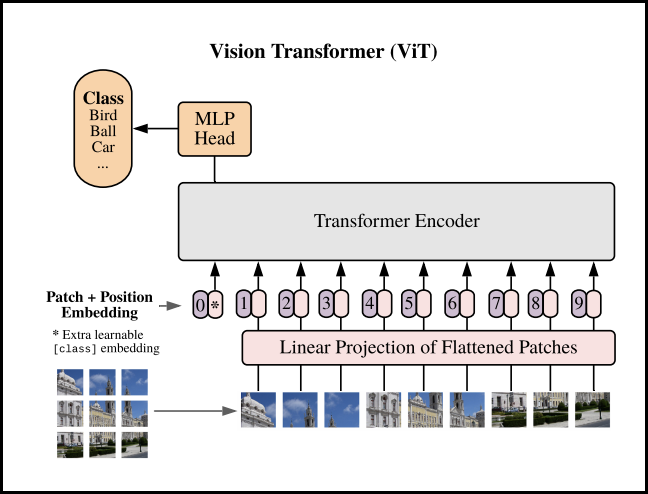
\includegraphics[width=0.7\linewidth]{Honors_Thesis/Figures/3.2.png}
\end{center}
\caption{The Vision Transformer - model architecture \cite{DBLP:journals/corr/abs-2010-11929}.}
\label{fig:3.2}
\end{figure}

\subsection{Insect Detection and Classification Models}
The on-site system that is responsible for sending insect data and running the Machine Learning models uses advanced AI detection and classification models to locate objects in the image returned from the camera and assign classes to those detections based on an insect dataset \cite{helton_luu_dowling_2022}.

The dataset used combines manually sourced images of bee flies, the IP102 dataset \cite{8954351}, and the EU Moths dataset \cite{DBLP:conf/gi/KorschBD21}. The 2,205 image dataset was manually annotated for the detection model to work. The final detection model was implemented using a Detection Transformer (DETR) as opposed to yolov5 due to its higher accuracy \cite{li2022dndetr}. Similarly, the final classification model was implemented using a Vision Transformer instead of a CNN to improve accuracy in recognizing minuscule differences between insect specifies. Using both models, the automated system can produce annotated images and extract data from them, as shown in Fig \ref{fig:3.3}.

\begin{figure}[H]
\begin{center}
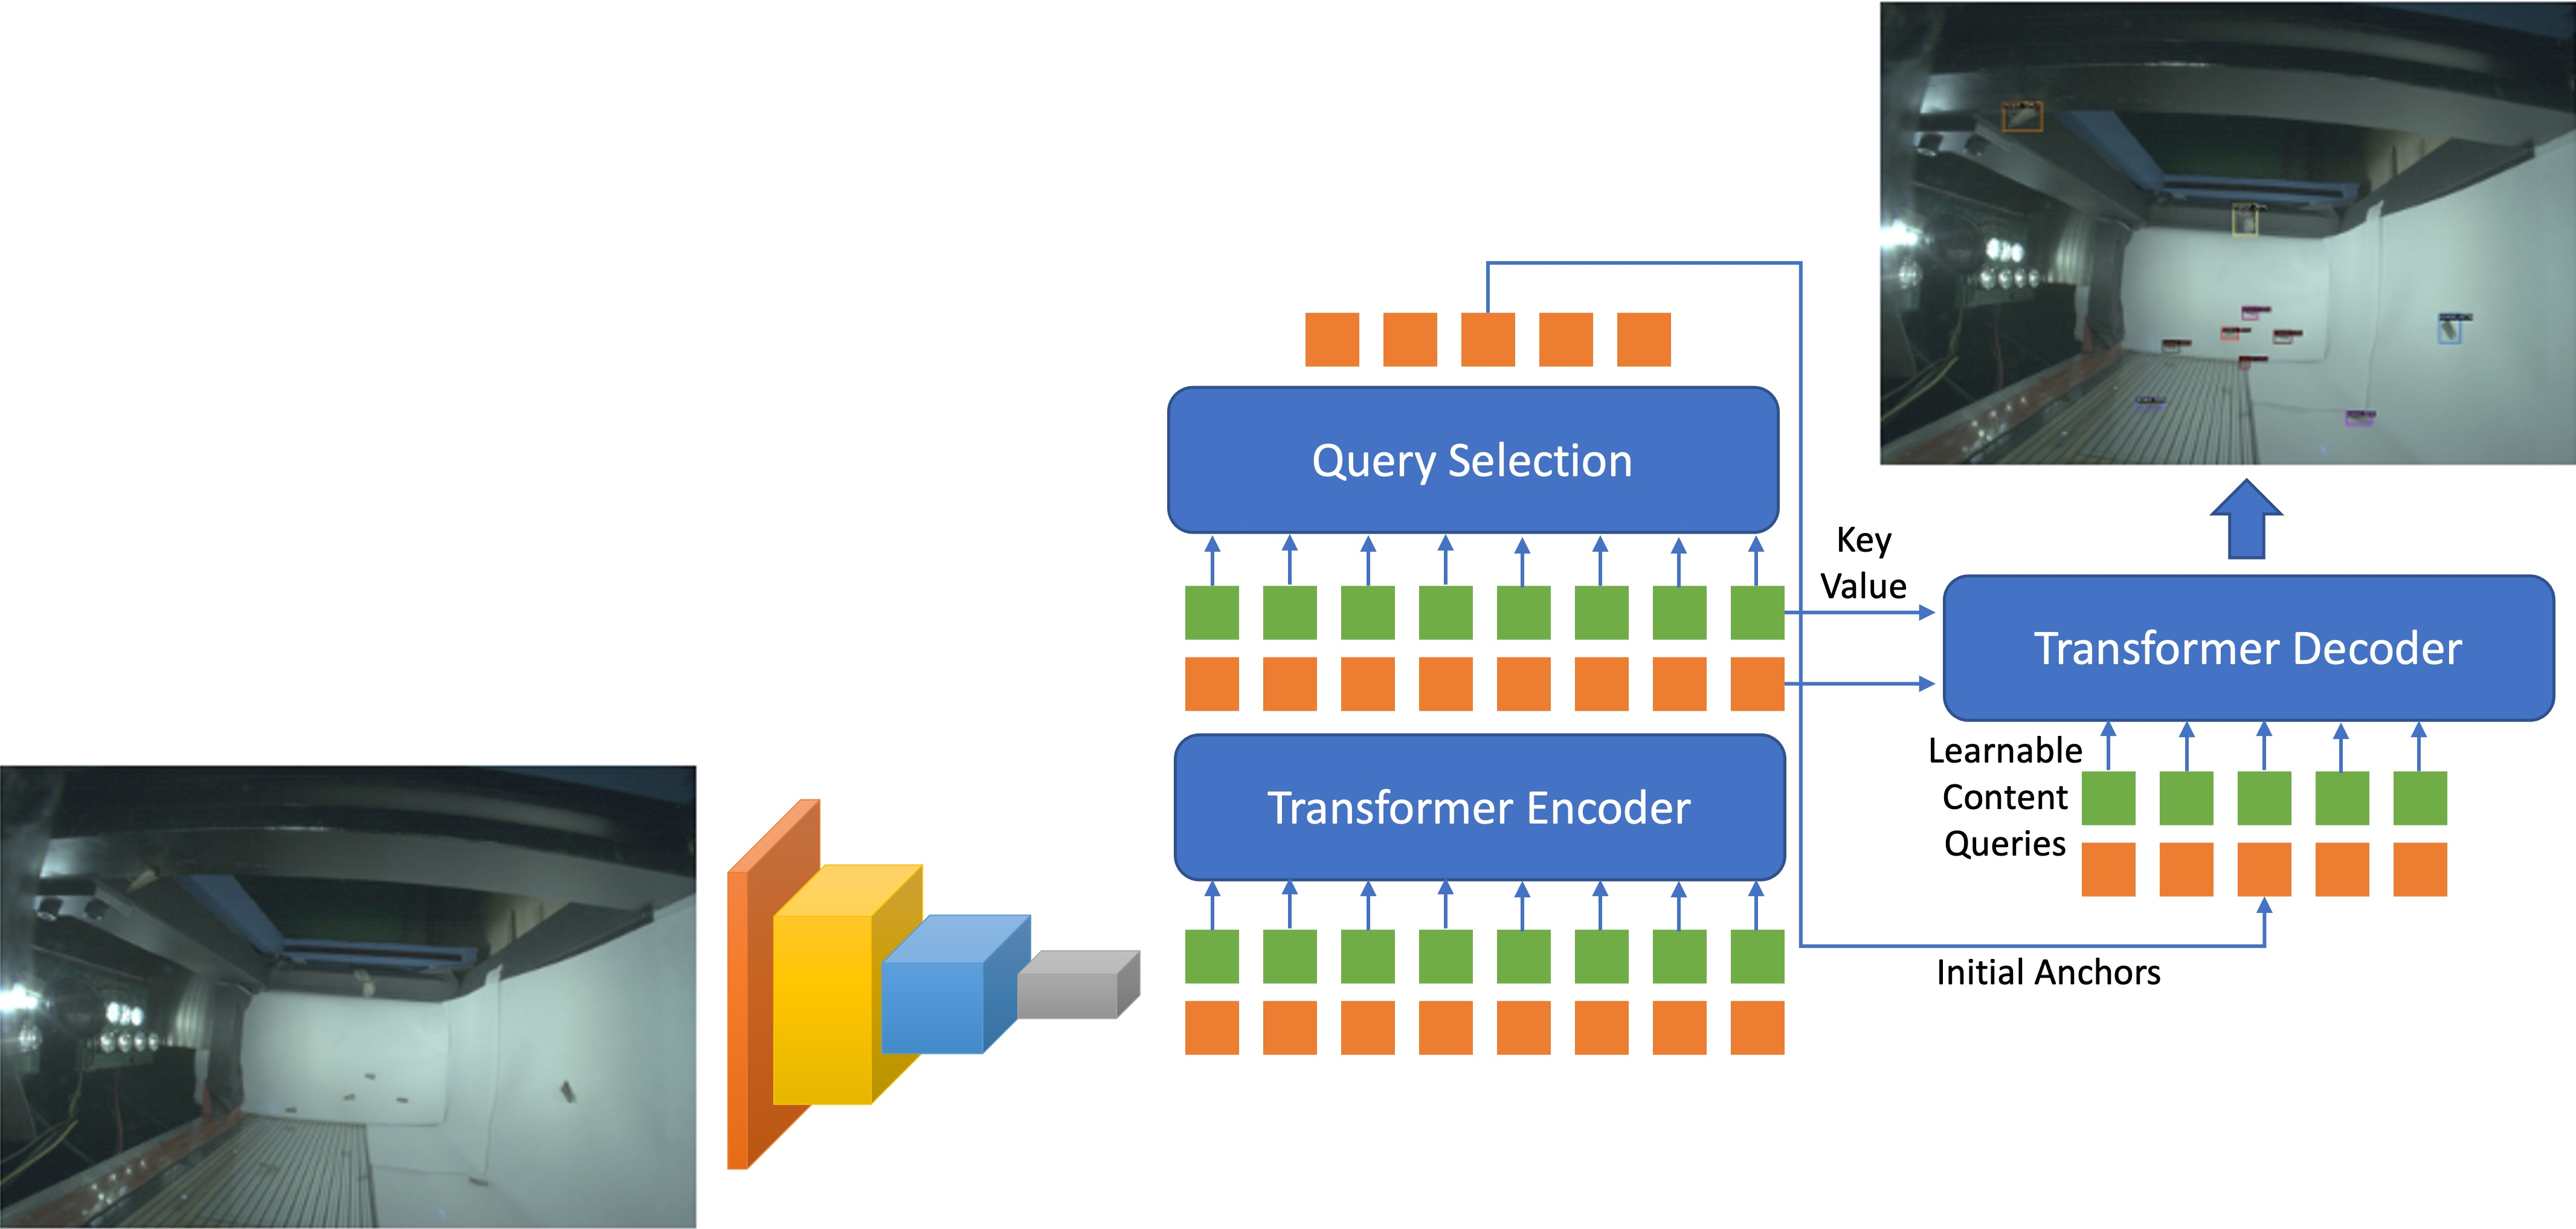
\includegraphics[width=1.0\linewidth]{Honors_Thesis/Figures/3.3.jpg}
\end{center}
\caption{Bug system transformer diagram.}
\label{fig:3.3}
\end{figure}

\section{Generative Pretrained Transformer (GPT)}
The Generative Pretrained Transformer (GPT) is a groundbreaking large language model (LLM) based on the Transformer architecture that leverages unsupervised learning for natural language understanding tasks. The underlying principle of GPT is a two-step process that involves unsupervised pre-training followed by supervised fine-tuning. Initially, the model is trained on a large unannotated text corpus to learn a general language representation. Subsequently, it is fine-tuned on specific, smaller labeled datasets for targeted tasks \cite{radford_narasimhan_salimans_sutskever}.

The GPT model employs a variety of masked language modeling called ``masked multi-head self-attention," which allows it to scale to longer sequences and capture long-range dependencies more effectively than traditional recurrent neural networks (RNNs). The Transformer architecture at the core of GPT enables the model to process input tokens in parallel, resulting in improved computational efficiency and scalability compared to RNNs and LSTMs.

A key aspect of GPT's success is its ability to achieve state-of-the-art performance across various natural language understanding tasks, including sentiment analysis, natural language inference, and question answering. By leveraging a generative language model for unsupervised pre-training and fine-tuning for specific tasks, GPT outperforms previous models by a significant margin \cite{radford_narasimhan_salimans_sutskever}.

As GPT has evolved through different versions, such as GPT-3.5 and GPT-4, it has experienced significant improvements in model size, architecture, parameters, and performance. Each new version incorporates advancements in training techniques, data sources, and architectural refinements that enhance language understanding capabilities. Fig \ref{fig:3.4} shows the enormous gap in the number of parameters between GPT-4 and previous models.

\begin{figure}[H]
\begin{center}
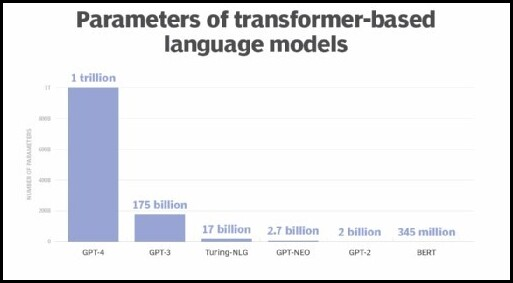
\includegraphics[width=0.8\linewidth]{Honors_Thesis/Figures/3.4.jpg}
\end{center}
\caption{Chart of No. of Parameters for multiple LLMs \cite{kerner_2023}.}
\label{fig:3.4}
\end{figure}

\subsection{Prompt Engineering}
Prompt engineering is the development and refinement of input prompts to guide the behavior of language models. It involves crafting the input text to effectively communicate the desired task to the model and elicit the desired response. Prompt engineering is important because the quality of the prompt can significantly impact the model's performance.

The choice of examples, the phrasing of the task, and other elements of the prompt can influence the model's understanding and output. For instance, in few-shot learning, the prompt may include a few examples of the task to be performed, followed by the specific instance on which the model should generate a response. Prompt engineering is still an active area of research, with development being done to create more effective prompts and evaluate model performance in various tasks for comparison \cite{prompt_eng_1, liu-etal-2021-noisy}.


\chapter{Implementation}

This chapter covers the implementation process behind the user-facing application that combines the insect detection and classification model with an emulated agriculture and insect expert using GPT. The implementation process was divided into three major components: the backend, the frontend, and the AI Chat feature. 

The backend component is responsible for the application's core functionality, including the integration of the insect detection and classification model with the database management system. The backend was developed using TypeScript and ExpressJS framework, which provided a solid foundation for building scalable and robust web applications. For database management, we've opted for Firebase, a highly-regarded open-source solution by Google known for its dependability and data integrity.

The frontend component is responsible for the visual representation and interaction of the application with the user. It includes the development of the user interface, which was designed to be intuitive and user-friendly, allowing farmers to access the features they need easily. The frontend was implemented using modern web technologies and packages such as HTML, CSS, TypeScript, Recharts, and more, with the React framework being used as the primary tool for development.

The AI Chat feature is the most innovative component of the application. It integrates OpenAI's GPT-3.5 model to provide personalized responses and recommendations based on the unique input from each farmer. This feature was developed using Typescript and the OpenAI API. Implementing this feature required extensive testing of various prompts to ensure its effectiveness as an emulator of agricultural expertise.

\section{Backend}

The backend for the Insect Detection Server project is primarily responsible for managing the database, which stores detections and related data from the on-site machines, and maintaining the Application Programming Interface (API). The project's API is a service between multiple applications that essentially exposes routes to the frontend to read from the database and exposes routes for the on-site machines to write data to the database.

\subsection{Database}

The original design of this work had several goals in mind, which included creating an interface for farmers to access their pest-related data and connecting on-site machines running computer vision models responsible for insect detection and classification. Since there were no requirements for complicated queries on the stored data, a NoSQL approach with high scalability was preferred, and Google Firebase's FireStore Database met those demands better when compared to an alternative such as MySQL \cite{clark_2022}. The importance of designing the database schema lies in matching the payloads of the requests we send from other applications through our API. As such, we chose to use a simplified JSON payload that contains the date of the detection, the image with the bounding boxes returned from the on-site machine, and the array of detection objects, including all of the insect detections/classifications from the model. As shown in Fig \ref{fig:4.1}, the structure of each detection within the detections array includes the date it was captured and the name and confidence score returned by classification.

\begin{figure}[H]
\begin{center}
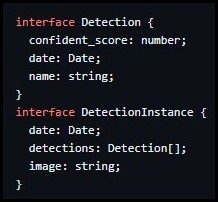
\includegraphics{Honors_Thesis/Figures/4.1.jpg}
\end{center}
\caption{TypeScript interface structures for the Detection and Detection Instance object used in the JSON payload and database schema.}
\label{fig:4.1}
\end{figure}

Within the FireStore Database, the types match those of the structures from Fig \ref{fig:4.1}. We store the image as a string rather than using a separate object storage service because we can convert our consistent 2K resolution images retrieved from the camera on the farm into Base64 strings, which are relatively easy to store and retrieve at smaller image sizes. Another concept specific to Firebase is ``collections," which are simply containers for ``documents," the unit of storage in Firebase \cite{google}. The main benefit of these collections is that they provide easy user-based data storage, as each user can have a unique collection of data of a similar structure. The structure of each detection document within our detections collection can be seen in Fig \ref{fig:4.2}.

\begin{figure}[H]
\begin{center}
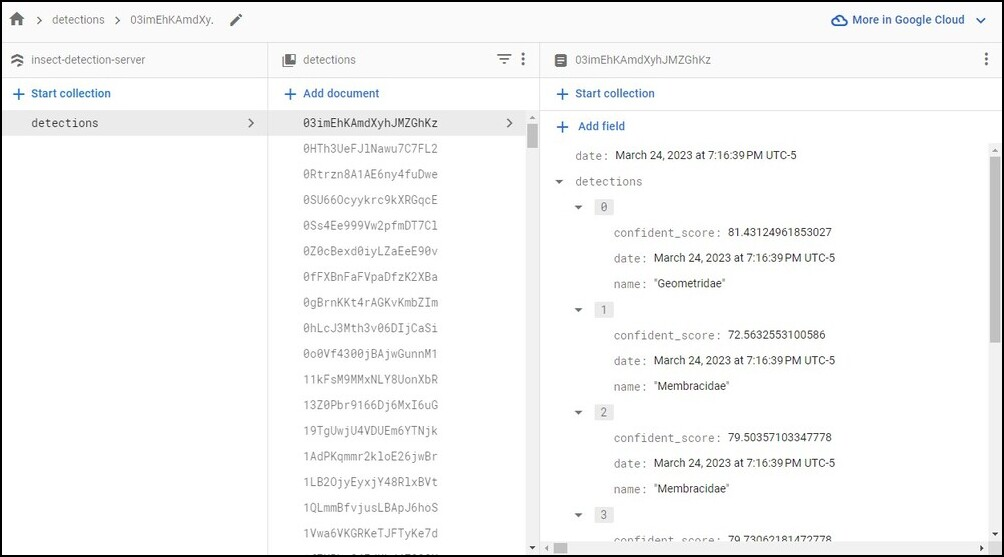
\includegraphics[width=1.0\linewidth]{Honors_Thesis/Figures/4.2.jpg}
\end{center}
\caption{Cloud FireStore Database data showcasing the detections collection and its child document structure. The document structure matches the interfaces from Fig \ref{fig:4.1}.}
\label{fig:4.2}
\end{figure}

\subsection{API}

The API serves as an interface between the frontend, on-site machines, and the database, allowing them to exchange data. It provides necessary routes to access and manipulate the data stored in FireStore. The API was developed in TypeScript using ExpressJS, a popular and powerful web application framework, and Firebase Functions, allowing us to run serverless functions responding to HTTP requests.

To implement the API, we defined the routes corresponding to the various actions the frontend and on-site machines can perform. The primary routes include fetching all detections for a specific day, fetching the latest detection data, and posting new detection data. The JSON response for a typical GET request from the frontend for a particular day's data is shown in Fig \ref{fig:4.3}. 

\begin{figure}[H]
\begin{center}
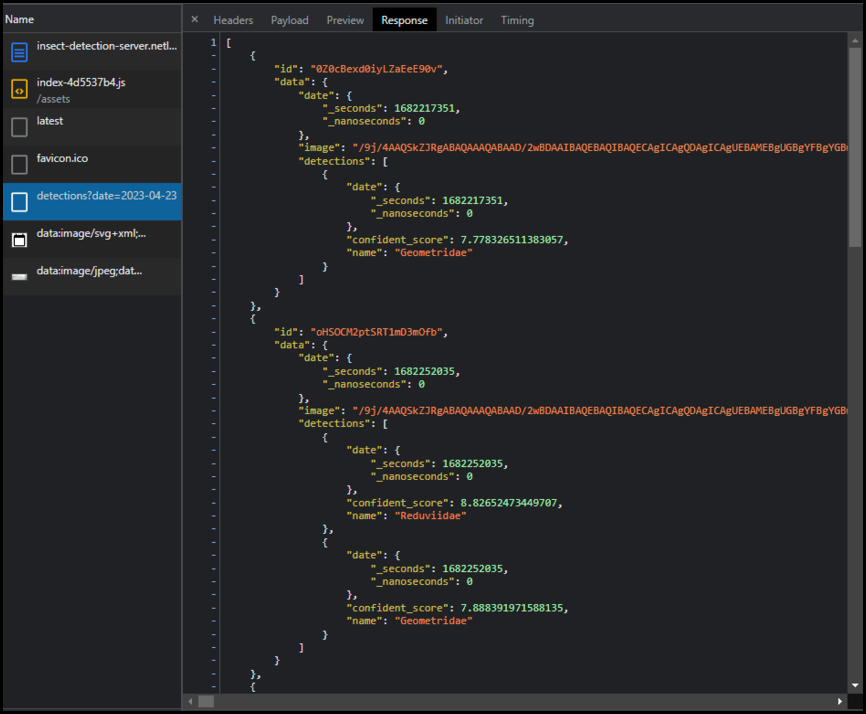
\includegraphics[width=1.0\linewidth]{Honors_Thesis/Figures/4.3.png}
\end{center}
\caption{JSON response example for a GET request from the frontend, returning all the detection data for a specific day.}
\label{fig:4.3}
\end{figure}

The on-site machines use the POST route to send new detection data to the database. These machines are responsible for running the insect detection and classification models, and they send the resulting data as a JSON payload. The response of the GET request is very similar to the payload of the POST request, as they contain the same data. A key difference is the format of dates due to their storage as milliseconds-since-epoch in the database. In Fig \ref{fig:4.4} we can see the POST request payload that matches up with the second detection document in the response from Fig \ref{fig:4.3}.

\begin{figure}[H]
\begin{center}
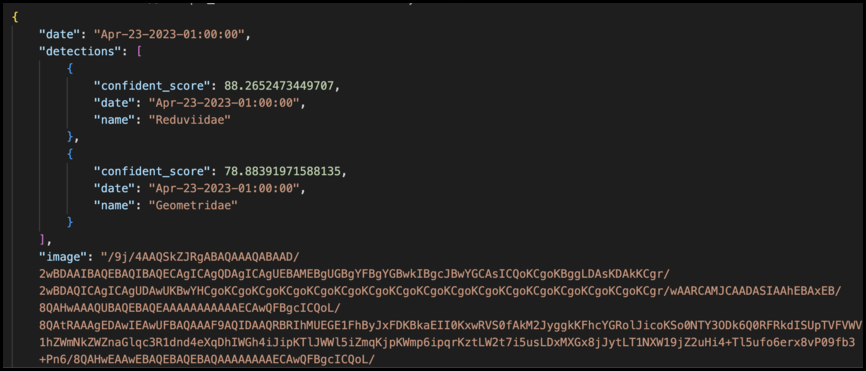
\includegraphics[width=1.0\linewidth]{Honors_Thesis/Figures/4.4.png}
\end{center}
\caption{JSON payload example for a POST request from the on-site machine. }
\label{fig:4.4}
\end{figure}

To handle these requests, we use Firebase Functions to define serverless functions that interact with the FireStore database. For example, we use a Firebase Function to fetch the latest detection data such that we can query the FireStore collection and return the most recent detection document. The sample Firebase Functions for handling the latest detection data request and saving detection data from the on-site machines are shown in Fig \ref{fig:4.5} and Fig \ref{fig:4.6}, respectively.

\begin{figure}[H]
\begin{center}
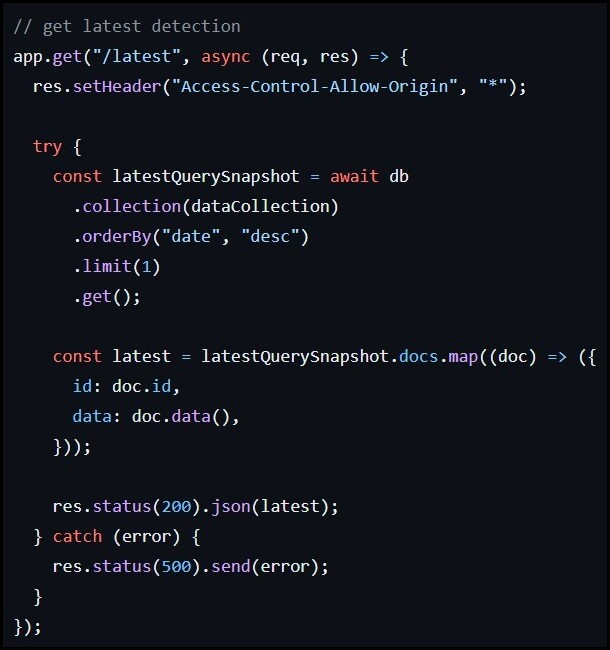
\includegraphics[width=0.8\linewidth]{Honors_Thesis/Figures/4.5.jpg}
\end{center}
\caption{Function for handling a GET request to fetch the latest detection data from the database.}
\label{fig:4.5}
\end{figure}

\begin{figure}[H]
\begin{center}
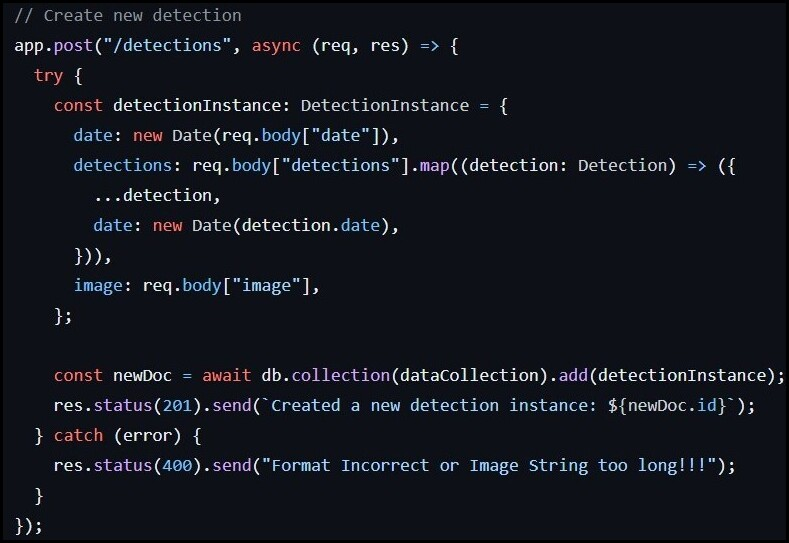
\includegraphics[width=1.0\linewidth]{Honors_Thesis/Figures/4.6.jpg}
\end{center}
\caption{Function for saving new detections to the database.}
\label{fig:4.6}
\end{figure}

Once the API and Firebase Functions were implemented, they could then be deployed to Firebase Hosting. This process involves bundling the API code and configuration files into a single package and uploading it to the Firebase servers. The deployment process is straightforward and ensures the API is accessible and scalable, handling many requests as needed. Ultimately, the API implementation facilitates seamless communication between the frontend, on-site machines, and the FireStore database. It enables efficient data retrieval and storage, ensuring a smooth user experience and accurate tracking of insect detection data over time.

\section{Frontend}

The frontend component was implemented using the React framework and TypeScript. React is a widely-used library for building user interfaces, while TypeScript adds static types to JavaScript, ensuring better code quality and maintainability. The frontend is deployed on Netlify, which automatically builds and deploys the application from the GitHub repository.

The primary goal of the frontend design was to provide an intuitive and user-friendly interface for farmers to monitor insect detections and classifications daily and review individual detection instances. To achieve this goal, we created a UI with a header row with a date picker in the center and an open chat button in the top right. The page's main content consists of a pie chart for the total insect detection statistics for the selected day, followed by images of detections throughout the day, which users can click left and right through. The pie chart is implemented using Recharts, a popular charting library for React.

Figure \ref{fig:4.7} presents the website UI with the pie chart at the top and the image with detections returned from the on-site machine at the bottom. The pie chart is tooltip-enabled, allowing users to see the average confidence percentage and the insect's name when they hover over a chart section.

\begin{figure}[H]
\begin{center}
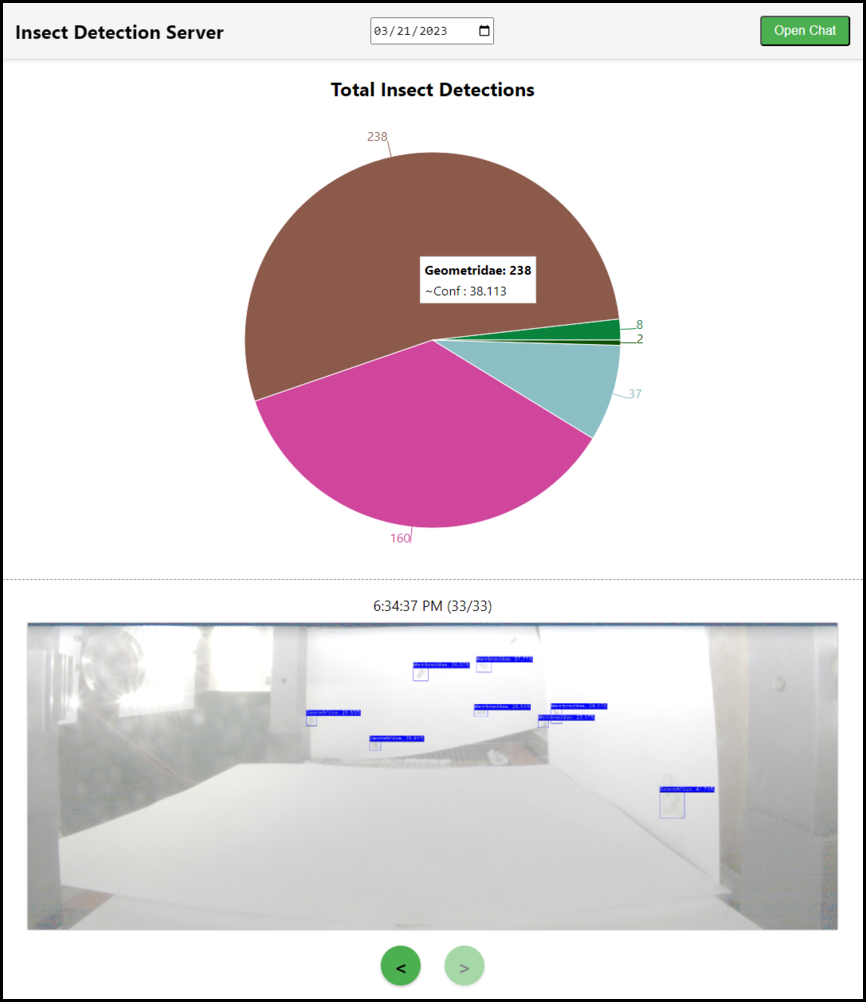
\includegraphics[width=1.0\linewidth]{Honors_Thesis/Figures/4.7.png}
\end{center}
\caption{The frontend user interface showcasing the pie chart with tooltip functionality and the image carousel for individual detections.}
\label{fig:4.7}
\end{figure}

\section{Artificial Intelligence Chat Feature}

The Artificial Intelligence chat feature is designed to provide farmers with personalized responses and recommendations based on their specific questions related to pests. To implement this feature, we integrated OpenAI's GPT-3.5 model using the OpenAI API and TypeScript. The decision to use GPT-3.5 over OpenAI's recently released GPT-4 was due to the superior speed and simplicity of GPT-3.5. However, due to its advanced reasoning, integrating GPT-4 could result in more advanced discussions on the implications of the insects' presence. To maintain the previous message history and enable the model to generate coherent and accurate responses, exchanged messages are saved during the conversation. 

The chat feature is accessible via a chat modal UI, as shown in Figure \ref{fig:4.8}, where users can converse with the AI about their pest concerns. The AI assistant can address various pest-related questions, from identification and potential impact to research and case studies and offering specific advice on control and management strategies tailored to the user's farm and crop conditions. By leveraging the advanced capabilities of GPT-3.5, the AI chat feature can provide detailed and accurate information, empowering farmers to make more informed decisions regarding pest management on their farms.

A limitation of the GPT model used, and large language models as a whole, is hallucinations. Hallucinations in AI are the generation of outputs that could be valid when they are factually incorrect. These phenomena can be explained by the limitations in the data the model was trained on. The issue with these hallucinations is their potential to mislead users since they can cause improper decision-making and a breakdown in trust in the model's other outputs \cite{gungor_2023}. We can see an example of GPT ``hallucination" in frames 1 and 2 of Fig \ref{fig:4.8} as most of the research articles referenced in its output do not exist. There are efforts to resolve these cases of hallucinations by implementing a validation step on GPT outputs. Still, the most effective response is transparency and disclosure of the model being used and its possible inaccuracies \cite{alkaissi_mcfarlane_2023}.

\begin{figure}[H]
\begin{center}
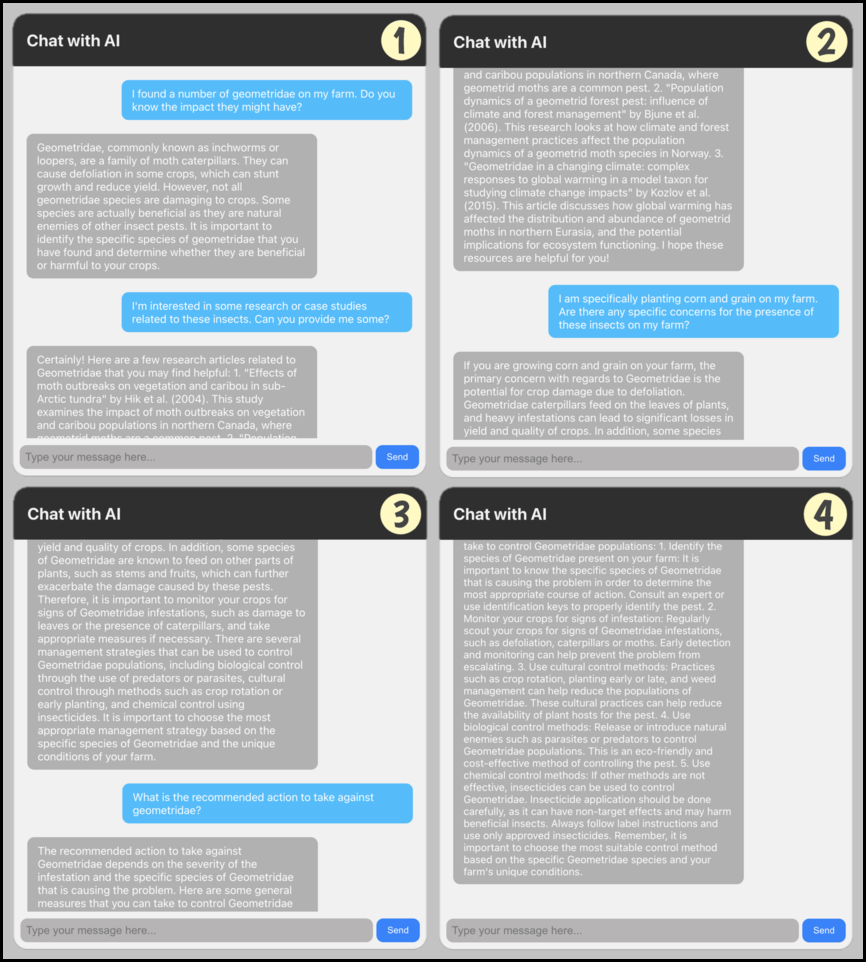
\includegraphics[width=1.0\linewidth]{Honors_Thesis/Figures/4.8.png}
\end{center}
\caption{The chat modal UI with an example conversation about pest-related questions.}
\label{fig:4.8}
\end{figure}

We employed prompt engineering techniques to guide the GPT-3.5 model in generating appropriate responses to ensure that the AI chat feature provides relevant and accurate information. In the API call, we specified the expertise in agriculture and insects as a system prompt so that the generated responses are appropriate and informed by agricultural knowledge. The importance of using a well-tested system prompt is to narrow the scope of the model's responses and promote only relevant conversations that are most beneficial to the typical user. We can see an example of the model's narrowed scope and promotion of relevant questions in Fig \ref{fig:4.9}. Figure \ref{fig:4.10} shows the example array of messages, a parameter in the API call's payload, including the system prompt.

\begin{figure}[H]
\begin{center}
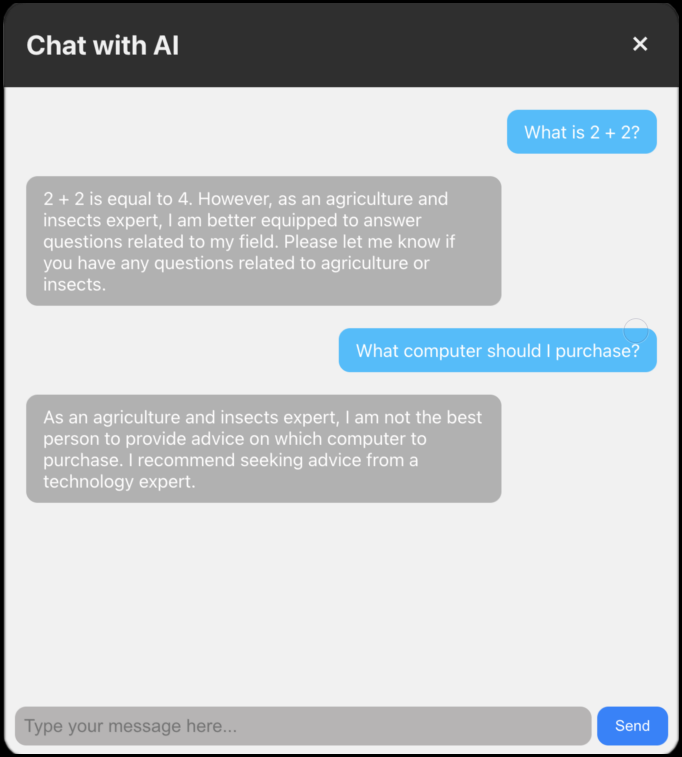
\includegraphics[width=0.8\linewidth]{Honors_Thesis/Figures/4.9.png}
\end{center}
\caption{Example conversation where the AI assistant exhibits narrowed scope.}
\label{fig:4.9}
\end{figure}

\begin{figure}[H]
\begin{center}
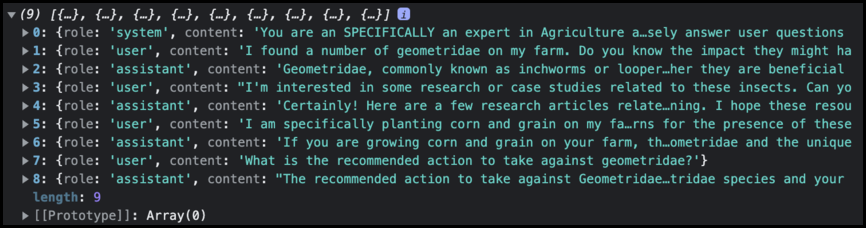
\includegraphics[width=1.0\linewidth]{Honors_Thesis/Figures/4.10.png}
\end{center}
\caption{Example messages parameter of payload for an API call to OpenAI's GPT-3.5 model with specified expertise in agriculture and insects.}
\label{fig:4.10}
\end{figure}

Implementing the AI chat feature required extensive testing and refining of prompts to ensure its effectiveness as an emulator of agricultural expertise. The result is an innovative and valuable addition to the application that helps farmers get quick and accurate information about their pest-related concerns, ultimately contributing to better decision-making in pest management.


\chapter{Conclusion}

The Insect Detection Server project demonstrates the potential of combining Artificial Intelligence, Computer Vision, and advanced language models to create a practical and accessible solution for pest management in the agricultural industry. By integrating the insect detection and classification model with OpenAI's GPT-3.5 model, the application provides farmers with a comprehensive tool that identifies insects on their farms and offers expert advice and personalized recommendations on pest management strategies.

The implementation of this project involved developing the backend, frontend, and AI chat feature, resulting in a user-friendly interface that allows farmers to monitor insect detections and engage in conversations about their pest concerns. The integration of GPT-3.5 API enables the AI chat feature to provide accurate and contextually relevant responses to user queries, emulating the expertise of a human agricultural specialist.

One of the primary benefits of this system is the potential for reducing pesticide use and hastening farmers' Integrated Pest Management plans, leading to improved crop yields and reduced environmental impacts. Furthermore, the techniques used in this research can be applied to a wide range of computer vision and user-facing data analytic applications, extending their potential implications beyond the agricultural industry.

Although the current implementation utilizes GPT-3.5, future work could explore integrating the more advanced GPT-4 model for even more advanced discussions on the implications of insect presence and potential pest management strategies. Additionally, further research could be conducted to refine the prompt engineering techniques and ensure the AI chat feature continues to provide relevant and accurate information in response to evolving agricultural practices and pest management strategies.

In conclusion, the Insect Detection Server project showcases the innovative application of Artificial Intelligence and Computer Vision technologies in addressing real-world problems farmers face. By providing a user-friendly and accessible tool for insect detection and expert advice, this project contributes to the ongoing efforts to improve the efficiency and sustainability of agricultural practices.


%bibliography is last chapter, before appendices
%use \nocite{} to put refs in bib that did not appear in the thesis

\chapter{Publications}


\textbf{\textit{CONDA: Continual Unsupervised Domain Adaptation Learning in  Semantic Scene Understanding}} (WACV 2023 - Submitted).


\bibliography{Honors_Thesis/thesis}


%BACK MATTER/APPENDICES
\appendix

%back matter are the microEP appendices
\chapter{Broader Impacts of Research}

\section{Applicability of Research Methods to Other Problems}
The innovative techniques and technology utilized in the creation of the Insect Detection Server hold great potential for application in various fields beyond agriculture. The incorporation of Computer Vision and AI for insect identification and classification, along with GPT-3.5's ability to simulate agricultural expertise, can be tailored to tackle various issues in different industries.

\begin{enumerate}
   \item Medical Imaging: In diagnostic scans, the Computer Vision methods employed for insect detection can be applied to medical imaging to identify and categorize medical conditions, such as tumors or lesions
   \item Environmental Conservation: The technology for wildlife monitoring and conservation initiatives can be modified. Utilizing computer vision to identify and track endangered species in their natural habitats allows conservationists to gather essential data on population dynamics and devise effective conservation strategies.
   \item Security and Surveillance: The computer vision model can be employed in security and surveillance systems to detect and recognize suspicious activities or individuals, thus enhancing security measures in public spaces and private properties.
   \item Customer Service: The implementation of GPT-3.5 as an ``online expert" can be expanded to other areas, including customer service and technical support. Companies can utilize AI chatbots to offer instant and personalized customer assistance, boosting customer satisfaction and reducing response times.
\end{enumerate}

\section{Impact of Research Results on U.S. and Global Society}
The Insect Detection Server has the potential to generate substantial positive impacts on both U.S. and global society, particularly within the agricultural sector.

\begin{enumerate}
    \item Improved Pest Management: The capacity to accurately identify and classify insects on farms enables farmers to implement targeted and timely pest control measures. This can result in more effective pest management, decreased crop damage, and heightened agricultural productivity.

    \item Reduced Pesticide Use: By supplying farmers with precise information about pest presence, the technology can help minimize the indiscriminate application of pesticides. This can reduce the environmental and health hazards associated with pesticide exposure.

    \item Enhanced Food Security: Better pest management and decreased crop losses contribute to improved food security by increasing the availability and affordability of food. This is especially crucial in regions where agriculture is a primary source of livelihood, and food security is a significant concern.

    \item Access to Expertise: The integration of GPT-3.5 as an ``online expert" offers farmers expert advice and guidance on pest management. This democratizes access to agricultural knowledge, particularly for small-scale farmers who may not have access to traditional agricultural extension services.
\end{enumerate}

\section{Impact of Research Results on the Environment}
The implementation of the Insect Detection Server can produce several positive environmental impacts:

\begin{enumerate}
    \item Reduction in Pesticide Pollution: By facilitating targeted pest management, the technology can decrease pesticide usage, reducing pesticide runoff into water bodies and soil contamination. This helps safeguard aquatic and terrestrial ecosystems from the detrimental effects of pesticides.

    \item Biodiversity Conservation: By curbing the indiscriminate application of pesticides, the technology can help protect non-target species, including beneficial insects such as pollinators, from pesticide exposure. This supports the conservation of biodiversity in agricultural environments.

    \item Sustainable Agriculture: The technology promotes sustainable agriculture practices by providing farmers with data-driven insights for pest management. This empowers farmers to make informed decisions that balance agricultural productivity with environmental responsibility.
\end{enumerate}

In conclusion, the Insect Detection Server holds the potential to promote more sustainable and eco-friendly agricultural practices. By harnessing AI and computer vision technologies, the research results can lead to enhanced pest management, reduced environmental impacts, and agricultural sustainability.

\chapter{Identification of All Software Used in Research and Thesis/Dissertation Generation}

Machine \#1:\\
Owner: Ahmed Moustafa\\\\
\begin{tabular}{ll}
Software\\
\hline
Ubuntu 18.0.4 \\
TypeScript \\
Open source web-development libraries \\
Google Firebase \\
OpenAI API \\
Netlify \\\\
\end{tabular}

Machine \#2:\\
Included CPU on the prototype bug system \\\\
\begin{tabular}{ll}
Software\\ 
\hline
Ubuntu 16.04 \\
Required scripts for system operation \\
\end{tabular}



\chapter{Plagiarism Check}
This thesis was created by Ahmed Moustafa. I attest that all work found in this document is my own. Any examples of repetition in other works is incidental and not plagiarized material.
\vspace{1in}
\makebox[1.5in]{\hrulefill}\\


\end{document}
